
% Make nice A4 pages for print:
%\usepackage{pgfpages}
%\pgfpagesuselayout{resize to}[a4paper,border shrink=5mm,landscape]

\beamertemplatenavigationsymbolsempty

\setbeamertemplate{bibliography item}[text]

\usepackage[type={CC},modifier={by-sa},version={4.0}]{doclicense}

\usepackage[utf8]{inputenc}
\usepackage{hyperref}
\usepackage{breakurl}
\usepackage{graphicx}
\usepackage{pgfplots}
\usepackage{pgf}
\usepackage{tikz}
\usetikzlibrary{positioning}
\usetikzlibrary{arrows}
\usetikzlibrary{decorations.markings}
\usetikzlibrary{calc}
\usetikzlibrary{matrix}
\usetikzlibrary{shapes}
\usetikzlibrary{decorations.pathmorphing}
\usetikzlibrary{fit}
\usetikzlibrary{backgrounds}
\usetikzlibrary{plotmarks}
\usepackage{stmaryrd}
\usepackage{listings}
\usepackage{pdflscape}
\usepackage{perpage}
\usepackage{appendixnumberbeamer}

%\usepackage[thmmarks,amsmath,amsthm]{ntheorem} % already included in beamer
\usepackage{thm-restate}

\usepackage[sort&compress,numbers]{natbib}  % to be have \citet, \citeauthor, \citeyear

\MakePerPage{footnote}

\tikzstyle{o}=[r,ppBlue]
\tikzstyle{r}=[thick,rectangle,align=center]
\tikzstyle{t}=[r,ppTrans] %,font=\bfseries]
\tikzstyle{dd}=[densely dashed]
\tikzstyle{n}=[r,ppBlue]
\tikzstyle{p}=[r,ppRed]
\tikzstyle{ppRed}  =[draw=red,  fill=  red!20]
\tikzstyle{ppBlue} =[draw=blue, fill= blue!20]
\tikzstyle{ppGreen}=[draw=green,fill=green!20]
\tikzstyle{ppTrans}=[draw=none, fill=none]

\usetheme{Warsaw}

\useoutertheme[subsection=true]{smoothbars}
%\useoutertheme[subsection=false]{miniframes}

\definecolor{bblue}{HTML}{D7DF01}	% yellow-ish actually, for better black/white printing
\definecolor{rred}{HTML}{C0504D}
\definecolor{ggreen}{HTML}{9BBB59}
\definecolor{ppurple}{HTML}{9F4C7C}
\definecolor{lightgray}{rgb}{0.3,0.3,0.3}
\definecolor{lightergray}{rgb}{0.9,0.9,0.9}
\definecolor{UniBlue}{RGB}{83,121,170}

\DeclareTextFontCommand\textintro{\normalfont\bfseries\itshape} % nice!
\newcommand{\intro}[2][]
{%
	\textintro{#2}%
}
\newcommand{\empha}[2][]
{%
	\emph{#2}%
}

%\theoremstyle{plain}
\newcounter{reqcounter}
\newtheorem{requirement}[reqcounter]{Requirement}

%setbeamercolor{structure}{fg=violet}

\makeatletter
\def\th@task{%
    \normalfont % body font
    \setbeamercolor{block title example}{bg=orange,fg=white}
    \setbeamercolor{block body example}{bg=orange!20,fg=black}
    \def\inserttheoremblockenv{exampleblock}
  }
\makeatother

\theoremstyle{task}
\newtheorem{task}{Task}

\newenvironment{assignment}%
{%\setbeamercolor{background canvas}{bg=violet}%
%\setbeamercolor{structure}{fg=cyan!90!black}%
 \setbeamercolor{frametitle}{bg=orange,fg=white}
\begin{frame}}%
{\end{frame}}%

\AtBeginSection[]{
  \begin{frame}
  \vfill
  \centering
  \begin{beamercolorbox}[sep=8pt,center,shadow=true,rounded=true]{title}
    \usebeamerfont{title}\insertsectionhead\par%
  \end{beamercolorbox}
  \tableofcontents
  \vfill
  \end{frame}
}




\pgfplotsset{compat=1.14}
\author{Markus Raab}


\date{4.5.2018}

\begin{document}

\renewcommand{\enquote}[1]{\emph{``#1''}} % Cannot be done earlier

%%%%%%%%%%%%%%%%%%%%%%%%%%%%%%%
\begin{frame}
	\titlepage
	\doclicenseThis
\end{frame}

\begin{frame}
	\frametitle{Organization}
	Next dates:
	\begin{description}
		\item[11.5.2018:] ???
		\item[18.5.2018:] guest lecture
		\item[25.5.2018:] \textbf{team exercise submitted} (1h earlier?)
		\item[1.6.2018:] lecture
		\item[8.6.2018:] lecture
		\item[15.6.2018:] last corrections of team exercise
		\item[22.6.2018:] test
	\end{description}
\end{frame}


\begin{frame}
	\frametitle{Popular Topics}
	\vspace{-0.5cm}
	\begin{multicols}{2}
	\begin{description}
	\item[4] validation
	\item[4] user interface
	\item[3] tools (benefits?)
	\color{gray}
	\item[3] testability
	\item[3] complexity reduction (when conf. needed?)
	\item[3] architectural decisions
	\color{black}
	\item[2] Puppet
	\color{gray}
	\item[2] modularity
	\item[2] environment variables
	\color{red}
	\item[2] documentation
	\item[2] configuration specification
	\color{gray}
	\item[2] command-line args\color{black}
	\color{black}
	\item[2] code generation
	\item[1] variability
	\item[1] self-description
	\item[1] round-tripping
	\color{gray}
	\item[1] early detection
	\item[1] introspection
	\item[1] dependences
	\item[1] auto-detection
	\color{red}
	\item[1] context-awareness
	\color{black}
	\item[1] administrators
	\end{description}
	\end{multicols}
\end{frame}

\begin{frame}
	\hspace*{-1cm}\includegraphics[width=\paperwidth]{dot/topics}
\end{frame}

\begin{frame}
	\frametitle{Modularity (Recapitulation)}
	\pause
	\Large
	\ExecuteMetaData[../book/backend.tex]{definition-modularity}
\end{frame}

\begin{frame}
	\frametitle{Vertical Modularity (Recapitulation)}
	\begin{columns}[c]
	\column{7cm}
	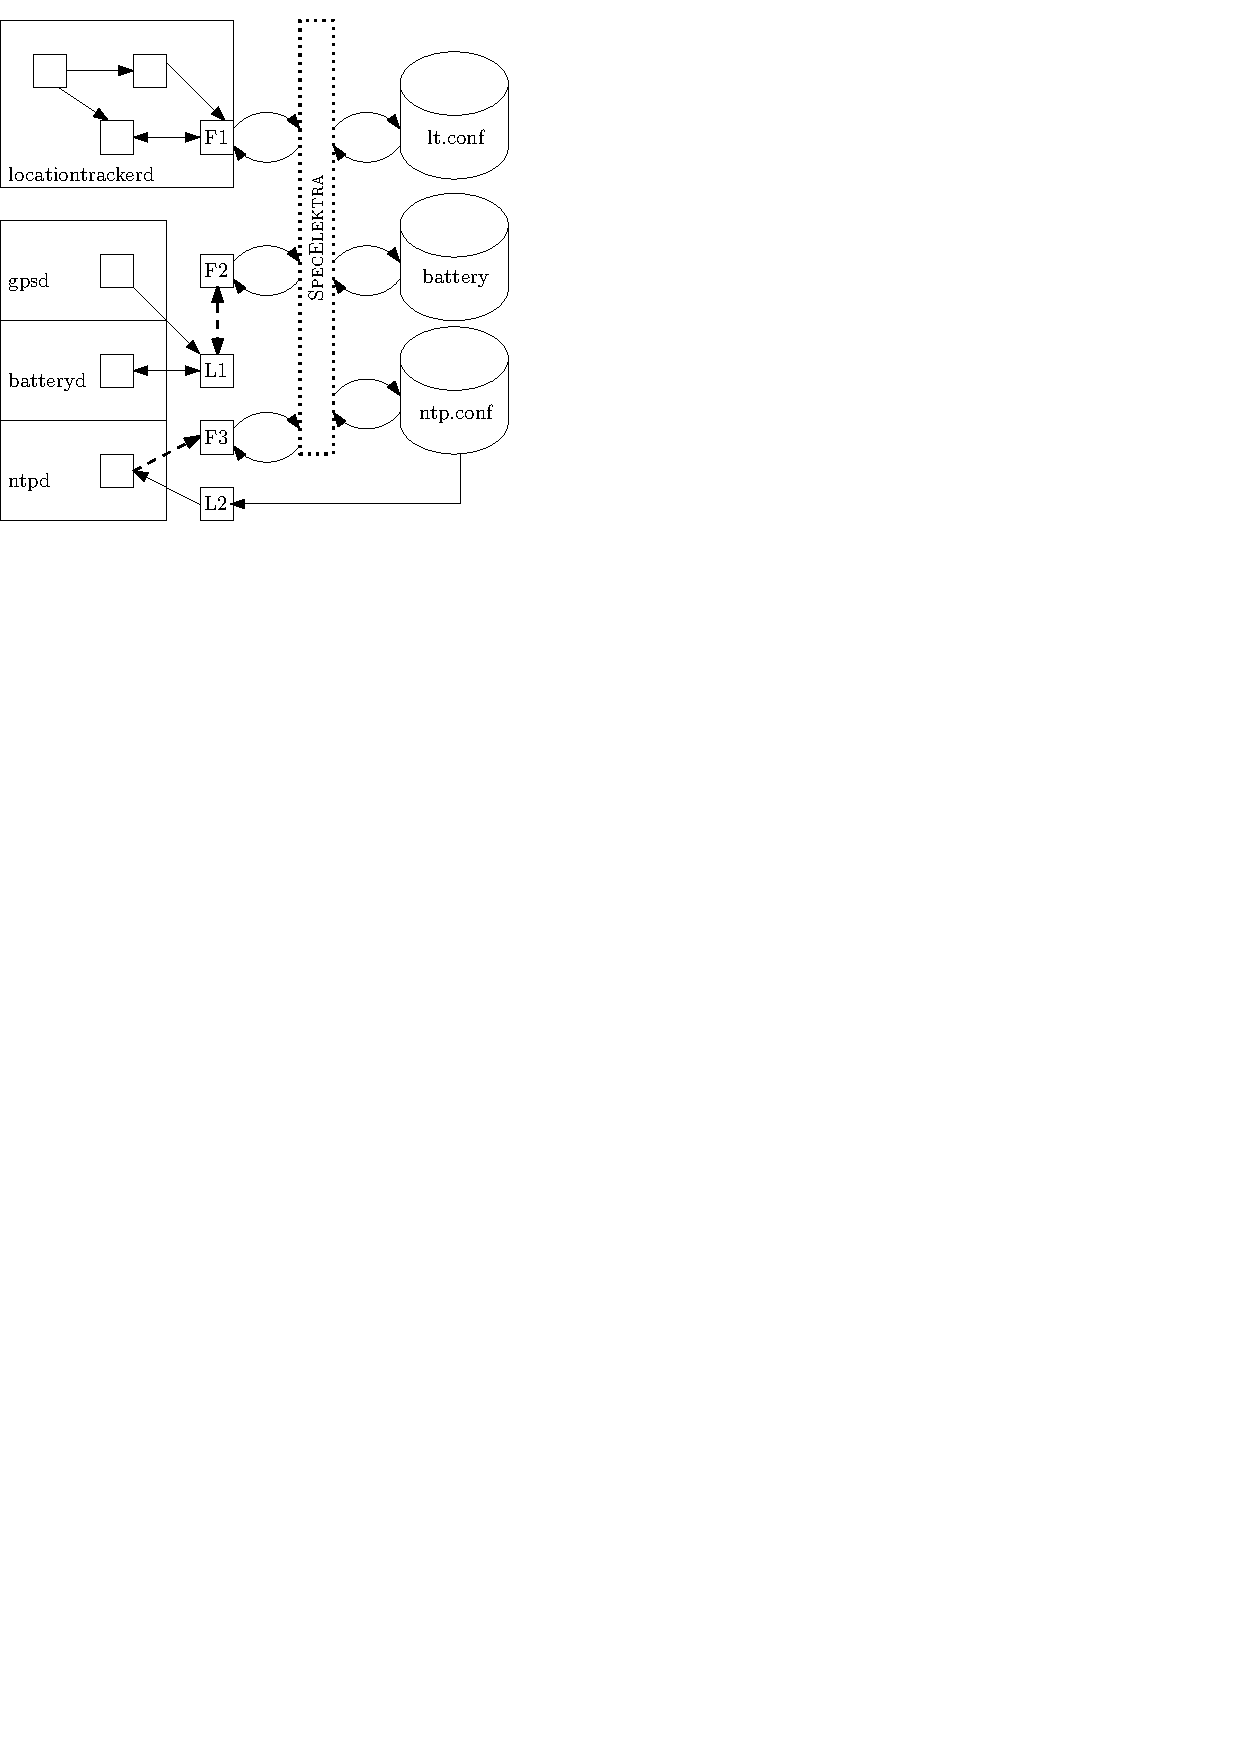
\includegraphics[scale=0.75]{verticalmodularity}
	\column{4cm}
	Needed to keep applications independently.

	Boxes are applications, cylinders are configuration files, F? are frontends or frontend adapters, L? are configuration libraries~\cite{raab2016improving}.
	\end{columns}
\end{frame}


\begin{frame}
	\frametitle{Introspection (Recapitulation)}
	\begin{task}
	What is internal and external specification?
	What is introspection?
	\end{task}

	\pause
	\vspace{1em}

	\begin{itemize}
	\item internal: within applications' source code
	\item unified get/set access to (meta*)-key/values
	\item access via applications, CLI, GUI, web-UI, ...
	\item access via any programming language (similar to file systems)
	\item GUI, web-UI can semantically interpret metadata
	\item needed as communication of producers and consumers of configuration
	\item essential for \intro[no-futz computing]{no-futz computing}~\citet{holland2001nofutz}
	\end{itemize}
\end{frame}

\begin{frame}
	\frametitle{Rationale (Recapitulation)}
	\begin{task}
	How to ensure that configuration access points match with present configuration settings?
	\end{task}

	\pause
	\vspace{1em}

	\textbf{Configuration Specification}:
	\begin{itemize}
	\item without specification you and others do not even know which settings are available
	\item needed for any further techniques we will discuss:
		\begin{itemize}
		\item code generation guarantees that configuration access points match with specification
		\item validation guarantees that configuration settings match with specification
		\end{itemize}
	\end{itemize}
\end{frame}

\begin{frame}
	Other Artefacts (Recapitulation):

	\pause

	\begin{itemize}
	\item examples (e.g., defaults)
	\item documentation
	\item auto-completion/syntax highlighting/IDE support
	\item tooling (GUI, Web UI)
	\item validation code
	\item configuration management tool code
	\end{itemize}
\end{frame}

\begin{frame}
	\frametitle{KeySet (Recapitulation)}

	The common data structure between plugins:
	\vspace{1cm}

	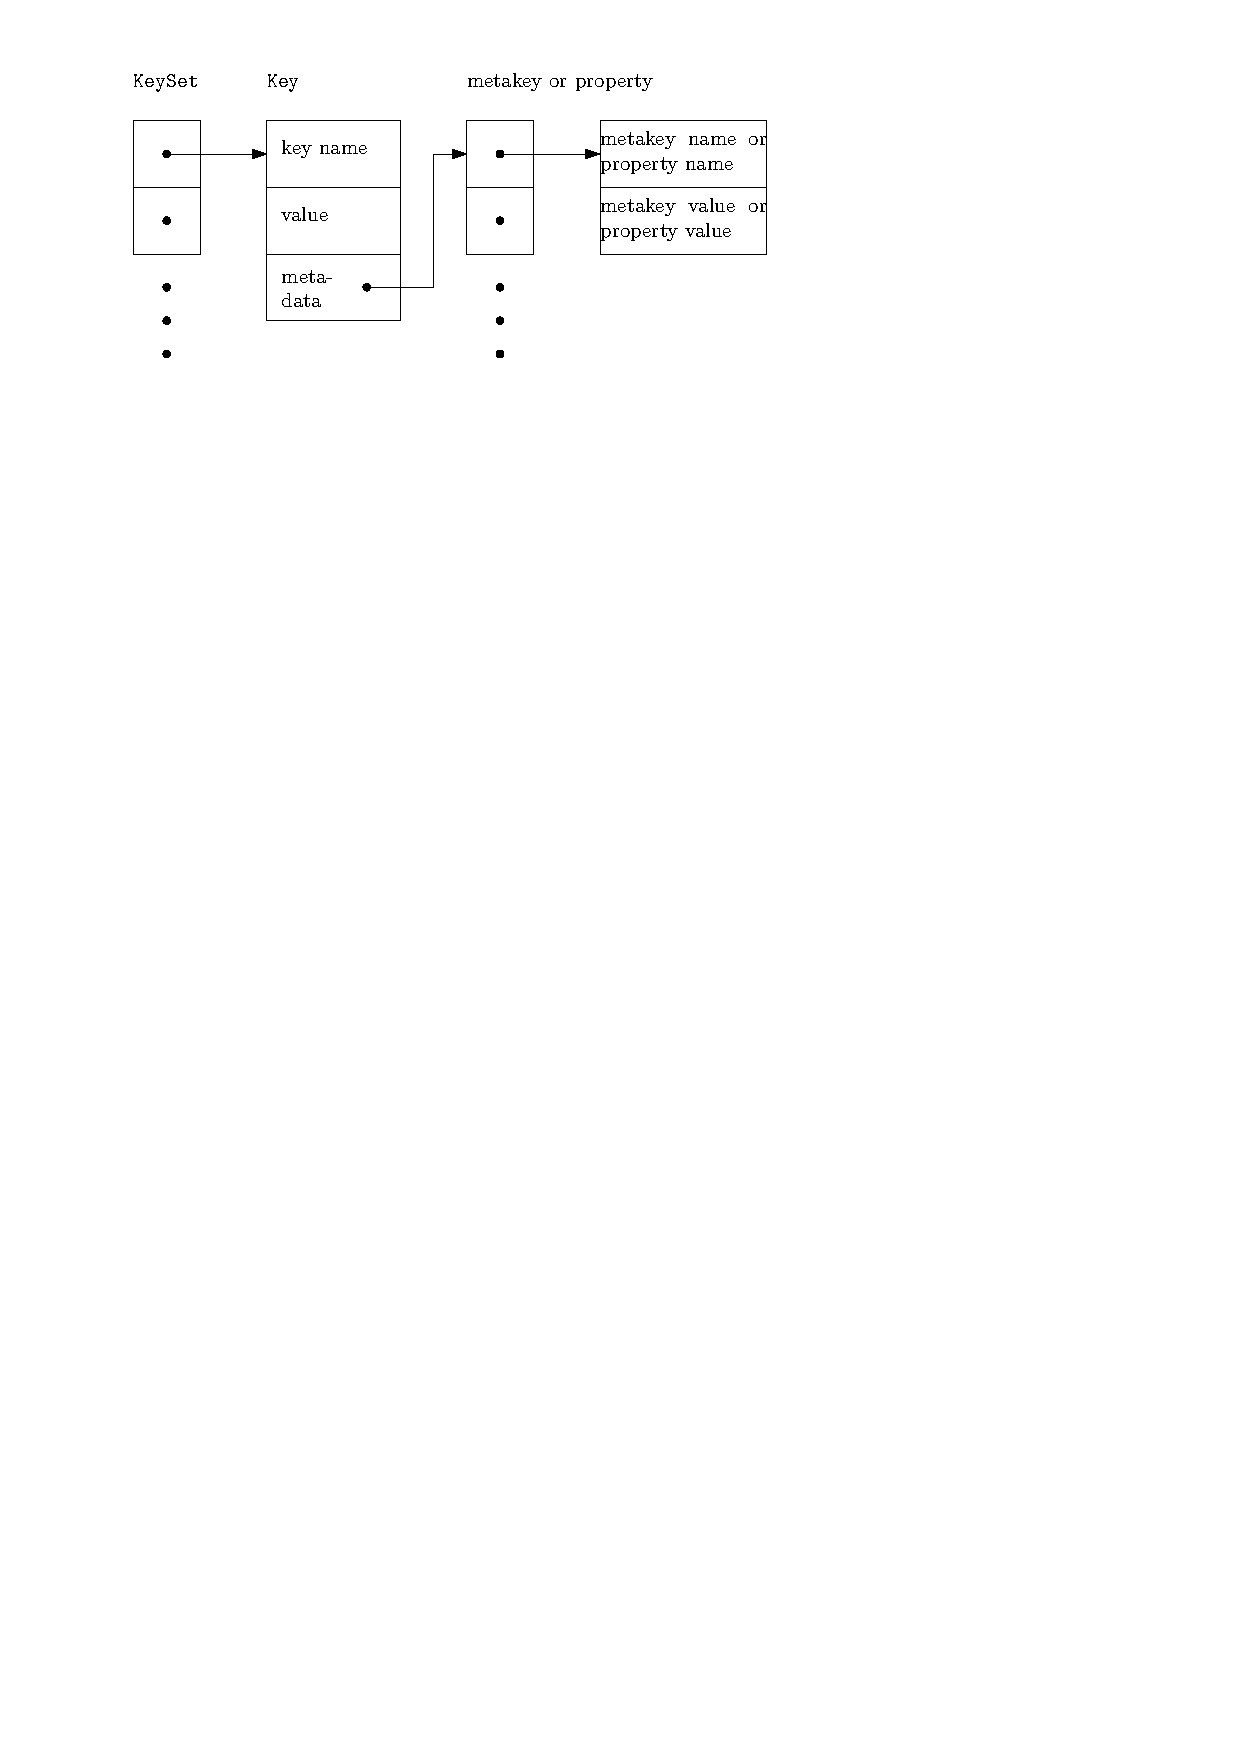
\includegraphics{keyset}
\end{frame}

\begin{frame}[fragile]
	\frametitle{KeySet Generation (Recapitulation)}
	\begin{alertblock}{Question}
	Idea: What if the configuration file format grammar describes source code?
	\end{alertblock}

	\pause

	key ^spec:/slapd/threads/listener^, with the configuration value ^4^ and the property $\property{default} \mapsto 1$:

	\begin{code}[gobble=4,language=Cpp]
	ksNew (keyNew ("spec:/slapd/threads/listener",
		       KEY_VALUE, "4",
		       KEY_META, "default", "1",
		       KEY_END),
	       KS_END);
	\end{code}

	\begin{alertblock}{Finding}
	We get source code representing the settings.
	\end{alertblock}
\end{frame}

\begin{frame}
	\frametitle{Introspection vs. Code Generation? (Recapitulation)}

	\pause

	\begin{description} %[leftmargin=0cm] %TODO: move left
	\item[$-$] more techniques for performance improvements with code generation
	\item[$+$] specification can be updated live on the system without recompilation
	\item[$+$] tooling has generic access to all specifications
 	\item[$+$] new features the key database (e.g., better validation) are immediately available consistently
	\end{description}

	\vspace{0.5em}

	\begin{alertblock}{Implication}
	We generally prefer introspection, except for a very thin configuration access API.
	\end{alertblock}
\end{frame}

\begin{frame}
	\frametitle{Testing (Recapitulation)}
	\begin{alertblock}{Question}
	What do we want to test?
	\end{alertblock}

	\pause

	\begin{itemize}
	\item That settings do what they should (devs and admins)
	\item That settings are properly validated (devs~\cite{xu2013blame})
	\item Regression tests~\cite{qu2008configuration}
	\pause
	\vspace{1em}
	\item Are all settings implemented?
	\item Are all settings used in tests?
	\item Are there unused settings in the code?
	\end{itemize}
\end{frame}

\begin{frame}
	\frametitle{Testing by developers? (Recapitulation)}

	\pause

	\begin{itemize}[<+-| alert@+>]
	\item ConfErr~\cite{keller2008conferr} uses models of key board layout, psychology and linguistics.
	Tool injects possible misconfiguration.
	\item Spex~\cite{xu2013blame} analyzes the source code to find misconfigurations.
	As by-product it extracts internal specifications (including transformation bugs).
	\item External specification can be directly used to generate test cases.
	\item Find unused configuration settings.
	\end{itemize}
\end{frame}

\begin{frame}
	\frametitle{When are settings used? (Recapitulation)}

	\pause

	\begin{description}[<+-| alert@+>]
	\item[Implementation-time] configuration accesses \index{implementation-time}
	are hard-coded settings in the sou\-rce code repository.
	For example, architectural decisions~\cite{zdun2007patterns} lead to impl\-ementation-time settings.

	\item[Compile-time] configuration accesses \index{compile-time}
	are configuration accesses resolved by the build system while compiling the code.

	\item[Deployment-time] configuration accesses \index{deployment-time}
	are configuration accesses while the software is installed.

	\item[Load-time] configuration accesses \index{load-time}
	are configuration accesses during the start of applications.

	\item[Run-time] configuration accesses \index{run-time}
	are configuration accesses during execution not limited to the startup procedure.
	\end{description}
\end{frame}

\begin{frame}
	\frametitle{Latent Misconfiguration (Recapitulation)}
	Phases when we can detect misconfigurations:
	\begin{itemize}[<+-| alert@+>]
	\item Compilation stage in configuration management tool
	\item Writing configuration settings on nodes
	\item Starting applications (load-time)
	\item When configuration setting is actually used (run-time)
	\end{itemize}

	\pause[\thebeamerpauses]

	\begin{alertblock}{Problem}
	More context vs. easier to detect and fix.
	\end{alertblock}
\end{frame}

\begin{assignment}
	\begin{task}
	Break.
	\end{task}
\end{assignment}


%%%%%%%%%%%%%%%%%%%%%%%%%%%%%%%%%%%%%%%%%% 
\section{Documentation}

\subsection{}


\begin{frame}
	\ExecuteMetaData[../book/motivation.tex]{documentation-inform}
\end{frame}

\begin{frame}
	There are at least two forms of documentation necessary:

	\begin{itemize}
	\item Explanations
	\item Examples
	\end{itemize}

	Generation helps to avoid duplication:

	\ExecuteMetaData[../book/motivation.tex]{documentation-req}
\end{frame}

\begin{frame}
	\begin{alertblock}{Question}
	How to avoid duplication between description text and other parts?
	\end{alertblock}

	\pause

	\begin{itemize}
	\item Render type and defaults into the documentation
	\item Render requirements and rationale into the documentation
	\item Use visibility to only show relevant configuration settings
	\end{itemize}
\end{frame}

\begin{frame}[fragile]
	\frametitle{Example}

	\begin{code}[gobble=4]
	[slapd/threads/listener]
	  check/range:=1,2,4,8,16
	  default:=1
	  description:=adjust to use more threads
	  rationale:=needed for many-core systems
	  requirement:=1234
	  visibility:=user
	\end{code}
\end{frame}

\begin{frame}
	\frametitle{Reevaluate specifications (Recapitulation)}

	In which situations should you reevaluate if a configuration setting (specification) is needed?

	\pause

	\ExecuteMetaData[../book/implications.tex]{reasons-adding}
\end{frame}


%%%%%%%%%%%%%%%%%%%%%%%%%%%%%%%%%%%%%%%%%% 
\section{Notification}

\subsection{}

\begin{frame}
	\frametitle{Notification Goals}

	\begin{enumerate}
	\item transient and persistent configuration settings always in sync~\cite{jin2014configurations}
	\item avoid polling of configuration settings
	\item integrate in already existing mechanisms (main loops)\footnote{Is one of the main reasons why most framework already integrate configuration settings.}
	\end{enumerate}

	\ExecuteMetaData[../book/motivation.tex]{req-consistency}
\end{frame}

\begin{frame}
	\frametitle{Conflicts}

	\pause

	\begin{itemize}
	\item If we write out configuration settings, we might conflict with settings recently written.
	\item Notification intensifies this problem (emergent misbehavior).
	\item Many conflicts can be resolved with a semantic 3-way merge.
	\end{itemize}
\end{frame}

\begin{frame}
	\frametitle{Semantic 3-way merge}

	The same problems happens when upgrading applications.

	\begin{itemize}
	\item System administrator changed the file.
	\item Package maintainer changed the file.
	\end{itemize}

	We can resolve many conflicts automatically, if we consider:
	\begin{itemize}
	\item the key/value structure (vs. line-based)
	\item the origin of both files
	\item the type of settings
	\end{itemize}
\end{frame}

\begin{frame}[fragile]
	\frametitle{Conflicts Example}

	\textbf{Ours:}
	\begin{code}[gobble=4,language=CfgElektra]
	slapd/threads/listener=4

	abc= \
		def
	\end{code}

	\textbf{Theirs:}
	\begin{code}[gobble=4,language=CfgElektra]
	abc = def
	slapd/threads/listener=8
	\end{code}

	\pause
	\textbf{Origin:}
	\begin{code}[gobble=4,language=CfgElektra]
	slapd/threads/listener=8
	abc=def
	\end{code}
\end{frame}

%%%%%%%%%%%%%%%%%%%%%%%%%%%%%%%%%%%%%%%%%% 
\section{Context-Awareness}

\subsection{}

\begin{frame}
	If you're a baker, making bread, you're a baker. If you make the best bread in the world, you're not an artist, but if you bake the bread in the gallery, you're an artist. So the context makes the difference.\par\raggedleft--- \textup{Marina Abramovic}
\end{frame}

\begin{frame}
	\ExecuteMetaData[../book/background.tex]{context-definition}
\end{frame}

\begin{frame}
	\frametitle{Types of Configuration}
	\begin{description}
	\ExecuteMetaData[../book/background.tex]{context-types}
	\end{description}
\end{frame}

\begin{frame}
	\hspace*{-1em}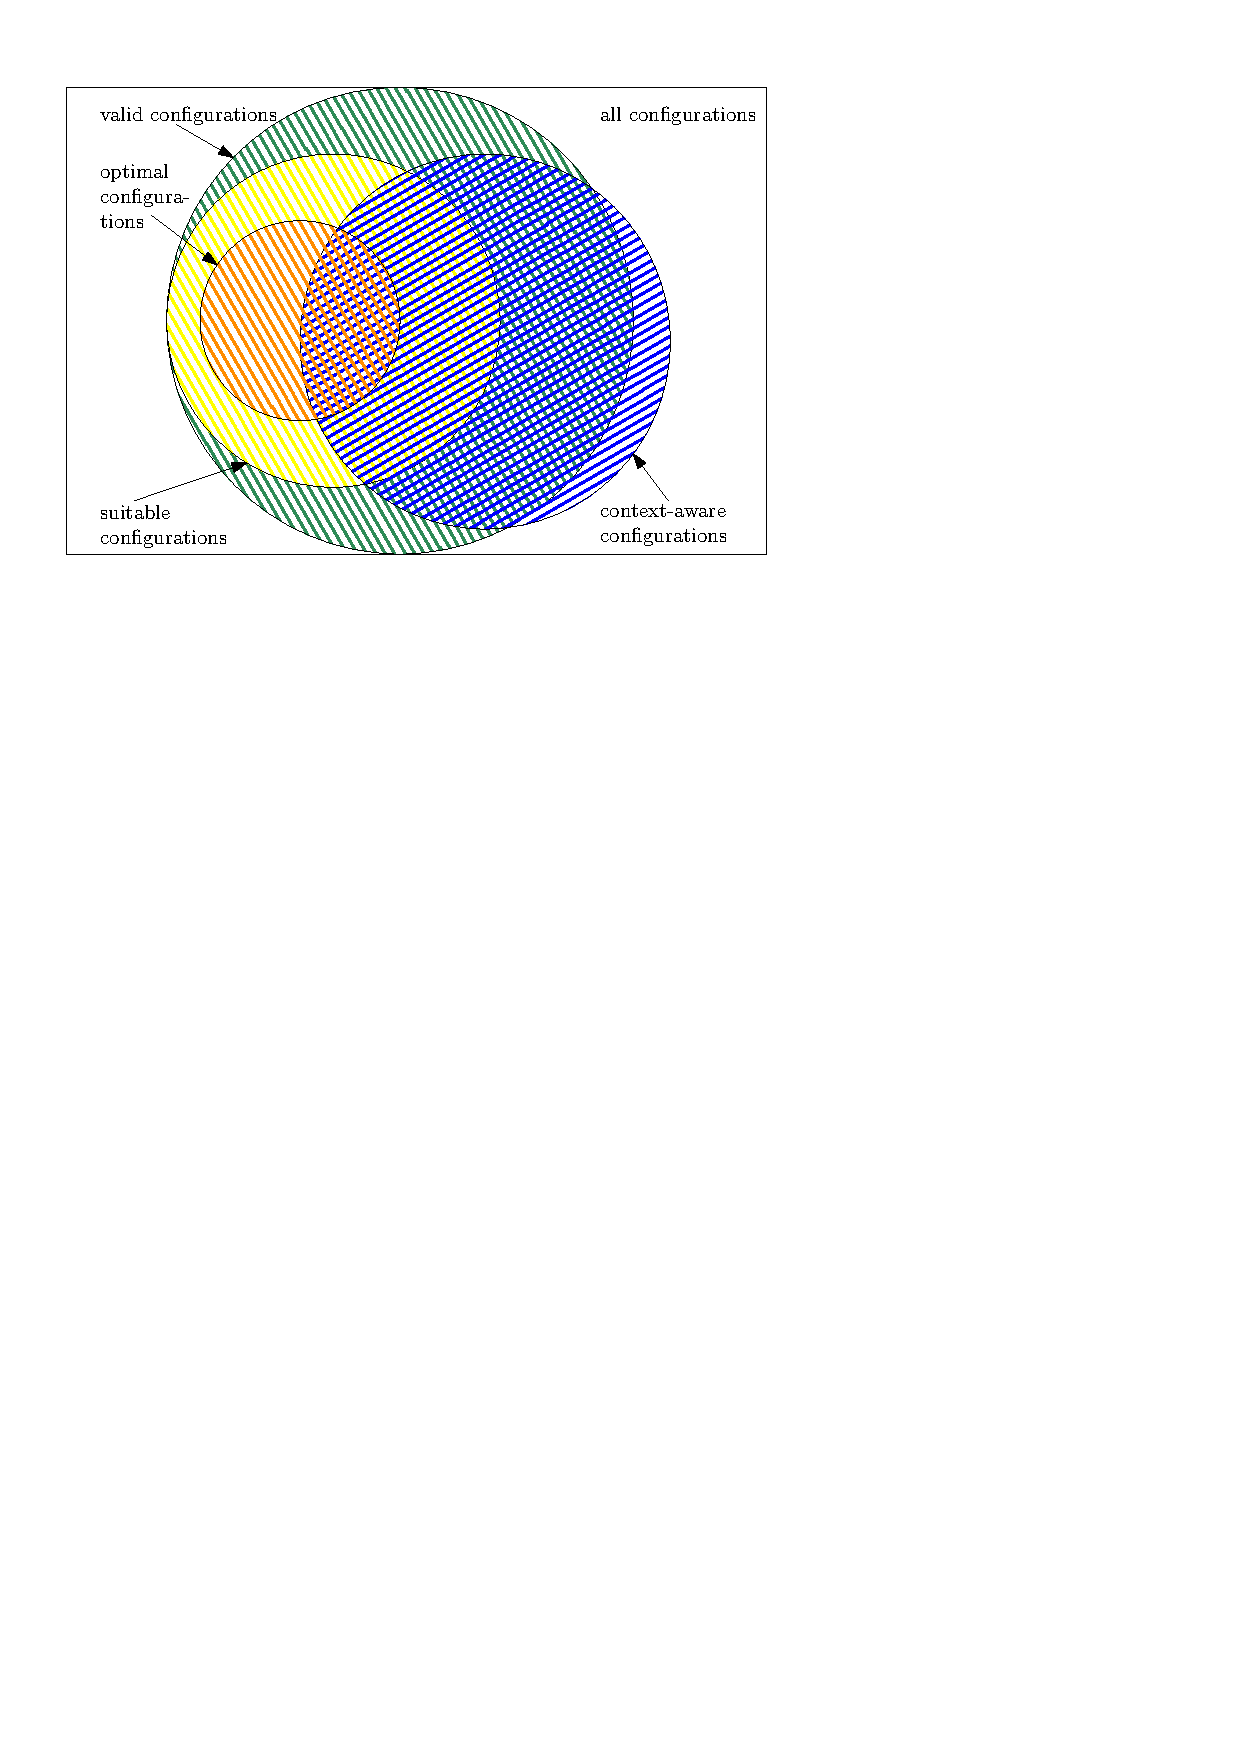
\includegraphics{configurations}
\end{frame}

\begin{frame}
	\frametitle{Viewpoints}
	\begin{description}
	\item[Sensors:] derive context from information sources of the system.
	Adding new context sensors increases the context available in a system.
	\ExecuteMetaData[../book/background.tex]{context-viewpoints}
	\end{description}
\end{frame}

\begin{frame}
	\frametitle{Cascading (Recapitulation)}
	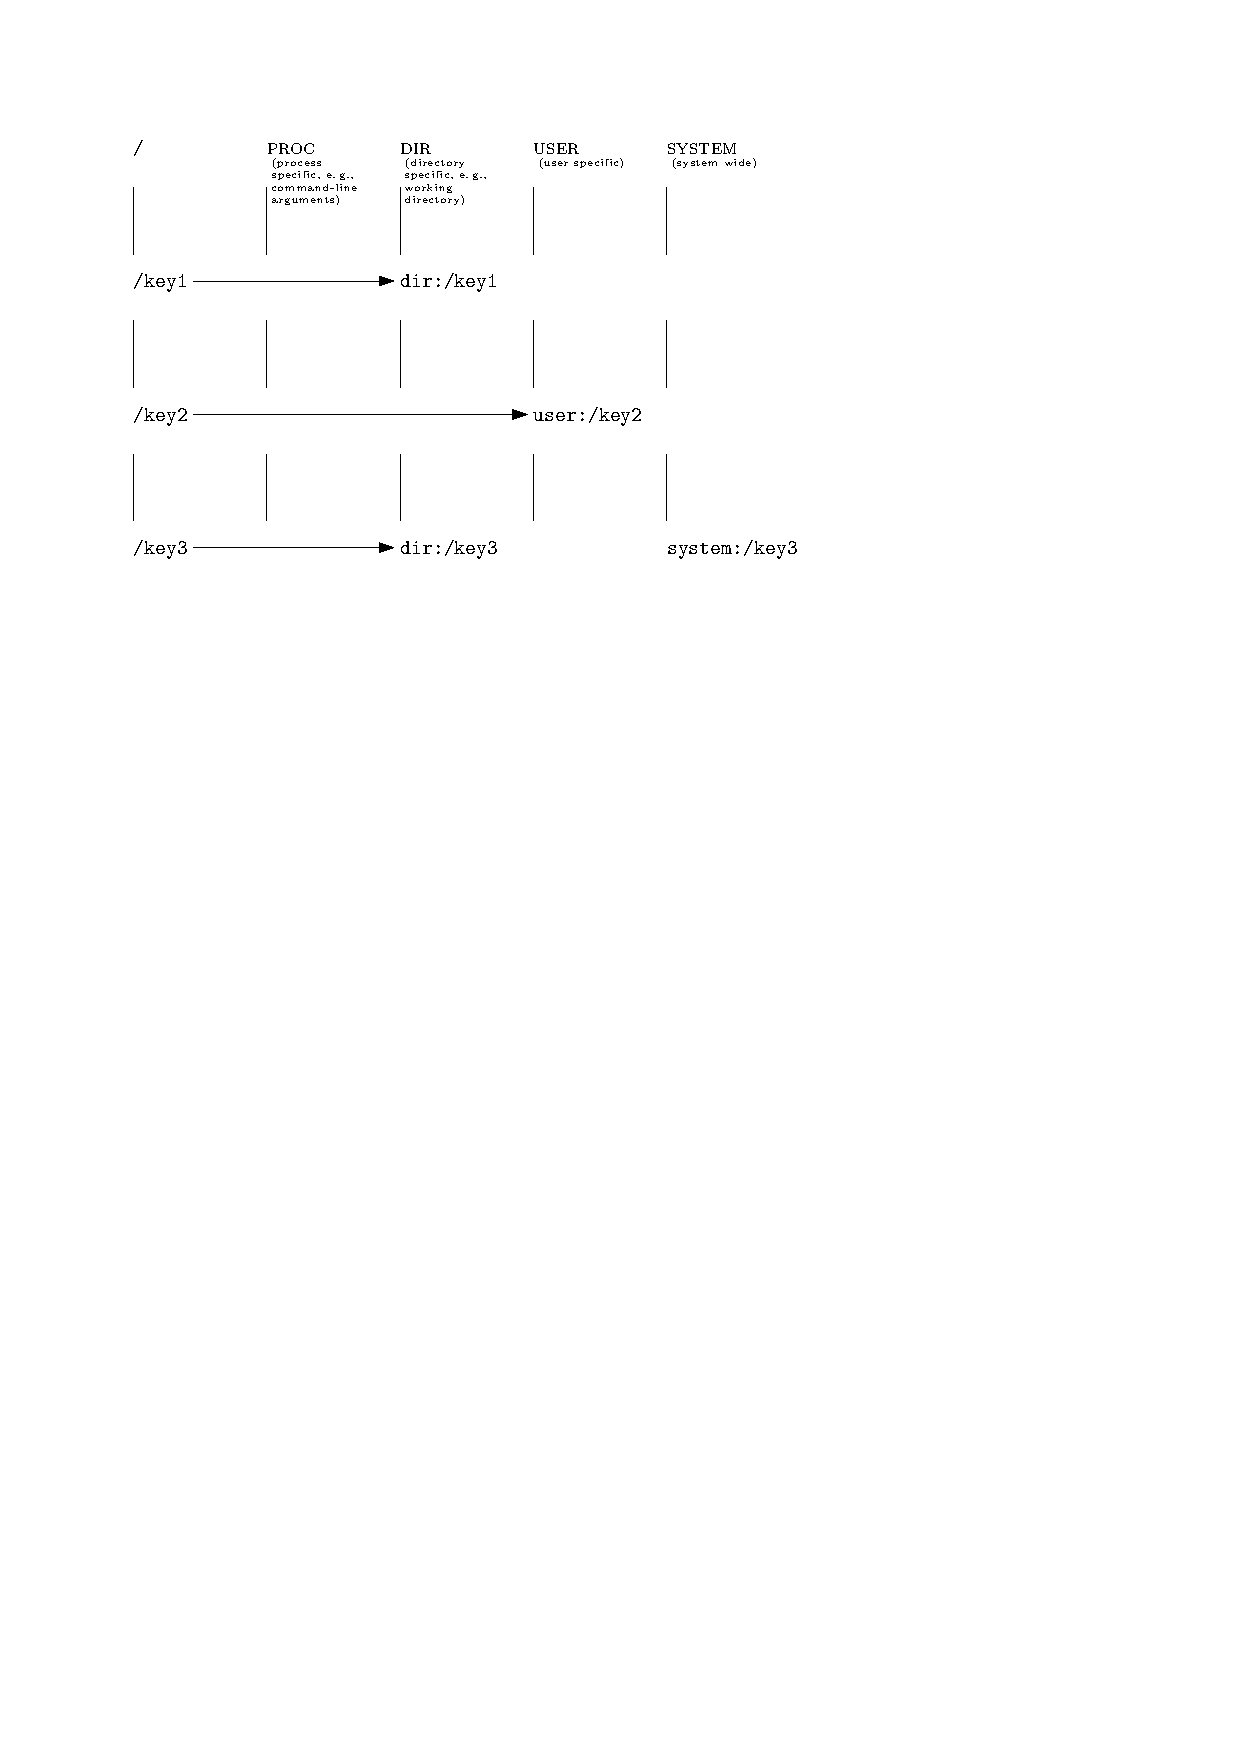
\includegraphics{cascading}
\end{frame}

\begin{frame}[fragile]
	\frametitle{Context-aware Lookup}

	\begin{itemize}
	\item
	Determine threads from CPUs:

	\begin{code}[gobble=4]
	[env/layer/cpu]
	  type:=long
	[slapd/threads/listener]
	  context:=/slapd/threads/%cpu%/listener
	\end{code}

	\item
	Determine vibration from sensors:

	\begin{code}[gobble=4]
	[phone/call/vibration]
	  type:=boolean
	  context:=/phone/call/%inpocket%/vibration
	\end{code}

	\item
	Determine proxy settings from network:

	\begin{code}[gobble=4]
	[env/override/http_proxy]
	  context:=/http_proxy/%interface%/%network%
	\end{code}
	\end{itemize}
\end{frame}


%%%%%%%%%%%%%%%%%%%%%%%%%%%%%%%%%%%%%%%%%% 
\section{Team Work}

\subsection{}

\begin{frame}
	\frametitle{Step 1 (5 min)}

	Familiarize yourself with one of the configuration systems:

	\begin{enumerate}
	\item environment variables (Factor 12)
	\item QSettings
	\item Apache Commons Configurations
	\item plist
	\item Windows Registry
	\item any other system you want to... (laptop)
	\end{enumerate}
\end{frame}

\begin{frame}
	\frametitle{Step 2 (45 min)}

	Come together in a group

	\begin{enumerate}
	\item decide who will create flip chart, moderate, and present
	\item explain the system you looked into
	\item explain what the system could do for the task
	\item create together an architecture that fulfils the goals
	\end{enumerate}
\end{frame}

\begin{frame}
	\frametitle{Goals}

	\begin{enumerate}
	\item configuration-management friendly
	\item early detection of misconfiguration
	\item smooth upgrades
	\item transient and persistent configuration consistent
	\item consistent documentation
	\item suitable and context-aware configurations
	\item reuse software as much as possible but integrate them nicely
	\end{enumerate}
\end{frame}

\begin{frame}
	\frametitle{Requirements}

	Design a camera system:

	\begin{enumerate}
	\item that is able to take single pictures and streams
	\item pluggable camera modules (lenses, image sensor, ...)
	\item should have camera profiles for different vendors
	\item a Web-UI that shows all configuration settings
	\item support remote configuration protocol (Web, SNMP, CMs, ...)
	\item time synchronization via NTP
	\item should be easily upgradeable (with fallback if the upgrade fails)
	\end{enumerate}
\end{frame}

\begin{frame}
	\frametitle{Tasks}

	\begin{enumerate}
	\item design and architecture of configuration settings
	\item design and architecture of configuration access
	\item design decisions (which languages, which software)
	\item explain how to ensure smooth upgrades
	\item provide documentation for operators (via IP)
	\item ensure synchronized, suitable and context-aware configuration
	\item reuse software as much as possible but integrate them nicely
	\end{enumerate}
\end{frame}





%%%%%%%%%%%%%%%%%%%%%%%%%%%%%%%%%%%%%%%%%% 
\nocite{raab2017introducing}

\appendix

\begin{frame}[allowframebreaks]
	\bibliographystyle{plainnat}
	\bibliography{../shared/elektra.bib}
\end{frame}

\end{document}


%TODO: add cliffhanger with preview for next time
